\chapter{Extracting Features from Unannotated Images}
\label{ch5}

This chapter is based on the following publications:
\begin{itemize}
    \item Zhou, Z., Sodha, V., Rahman Siddiquee M. M., Feng, R., Tajbakhsh, N., Gotway, M. B., \& Liang, J. (2019, October). Models genesis: Generic autodidactic models for 3d medical image analysis. In \textit{International Conference on Medical Image Computing and Computer-Assisted Intervention} (pp. 384-393). Springer, Cham.
    \item Zhou, Z., Sodha, V., Pang, J., Gotway, M. B., \& Liang, J. (2021). Models genesis. \textit{Medical image analysis}, 67, 101840.
\end{itemize}

% \section*{CRediT authorship contribution statement}

% I would like to thank all of the authors for their contributions and hard works. Vatsal Sodha: software, investigation, visualization. Jiaxuan Pang: software, investigation. Michael B. Gotway: resources, data curation, funding acquisition. Jianming Liang: conceptualization, methodology, formal analysis, investigation, resources, writing, supervision, project administration, funding acquisition. 

\newpage

\section{Background \& Motivation}

Recent years have featured a trend towards pre-trained image representations in computer vision, applied in increasingly flexible and task-agnostic ways for downstream transfer.
Transfer learning from {\em natural} images to {\em medical} images has become the \textit{de facto} standard in deep learning for medical image analysis~\citep{tajbakhsh2016convolutional,shin2016deep}, but given the marked differences between {\em natural} images and {\em medical} images, we hypothesize that transfer learning can yield more powerful (application-specific) {\em target} models from the {\em source} models built directly using medical images. To test this hypothesis, we have chosen chest imaging because the chest contains several critical organs, which are prone to a number of diseases that result in substantial morbidity and mortality, hence associated with significant health-care costs. In this research, we focus on Chest CT, because of its prominent role in diagnosing lung diseases, and our research community has accumulated several Chest CT image databases, for instance, LIDC-IDRI~\citep{armato2011lung} and NLST~\citep{national2011reduced}, containing a large number of Chest CT images. However, systematically annotating Chest CT scans is not only tedious, laborious, and time-consuming, but it also demands costly, specialty-oriented skills, which are not easily accessible. Therefore, we seek to answer the following question: {\em Can we utilize the large number of available Chest CT images without systematic annotation to train source models that can yield high-performance target models via transfer learning?} 

To answer this question, we have developed a framework that trains generic source models for 3D medical imaging. Our framework is {\em autodidactic}---eliminating the need for labeled data by self-supervision; {\em robust}---learning comprehensive image representation from a mixture of self-supervised tasks; {\em scalable}---consolidating a variety of self-supervised tasks into a single image restoration task with the same encoder-decoder architecture; and {\em generic}---benefiting a range of 3D medical imaging tasks through transfer learning.
We call the models trained with our framework Generic Autodidactic Models, nicknamed Models Genesis, and refer to the model trained using Chest CT images as Genesis Chest CT.
As ablation studies, we have also trained a downgraded 2D version using 2D Chest CT slices, called Genesis Chest CT 2D. For thorough performance comparisons, we have trained a 2D model using Chest X-ray images, named as Genesis Chest X-ray (detailed in~\tablename~\ref{ch5:tab:terminology}). 

Naturally, 3D imaging tasks in the most prominent medical imaging modalities (\eg CT and MRI) should be solved directly in 3D, but 3D models generally have significantly more parameters than their 2D counterparts, thus demanding more labeled data for training. As a result, learning from scratch simply in 3D may {\em not} necessarily yield performance better than fine-tuning Models ImageNet (\ie pre-trained models on ImageNet), as revealed in \figurename~\ref{ch5:fig:2D_3D_target_tasks}. However, as demonstrated by our extensive experiments in Sec.~\ref{ch5:experiments}, our Genesis Chest CT not only {\em significantly} outperforms learning 3D models from scratch (see \figurename~\ref{ch5:fig:random_initialization}), but also {\em consistently} tops any 2D/2.5D approaches including fine-tuning Models ImageNet as well as fine-tuning our Genesis Chest X-ray and Genesis Chest CT 2D (see \figurename~\ref{ch5:fig:2D_3D_target_tasks} and \tablename~\ref{ch5:tab:3d_2.5d_2d}). Furthermore, Genesis Chest CT surpasses publicly-available, pre-trained, (fully) supervised 3D models (see \tablename~\ref{ch5:tab:top_existing_models}). Our results  confirm the importance of 3D anatomical information and demonstrate the significance of Models Genesis for 3D medical imaging.

This performance is attributable to the following key observation: medical imaging protocols typically focus on particular parts of the body for specific clinical purposes, resulting in images of similar anatomy. The sophisticated yet recurrent anatomy offers consistent patterns for self-supervised learning to discover common representation of a particular body part (the lungs in our case). 
As illustrated in \figurename~\ref{ch5:fig:self_supervised_learning_framework}, the fundamental idea behind our self-supervised learning method is to recover anatomical patterns from images transformed via various ways in a unified framework. 

In summary, we make the following three contributions:
\begin{enumerate}
    \item A collection of generic pre-trained 3D models, performing effectively across diseases, organs, and modalities.
    \item A scalable self-supervised learning framework, offering encoder for classification and encoder-decoder for segmentation.
    \item A set of self-supervised training schemes, learning robust representation from multiple perspectives.
\end{enumerate}


%%%%%%%%%%%%%%%%%%%%%%%%%%%%%%%%%%%%%%%%%%%%
% \begin{landscape}
% \thispagestyle{empty}

\begin{sidewaystable}
\begin{threeparttable}[t]
\begin{center}
\footnotesize
\caption[Definition of Pre-trained Models, Proxy and Target Tasks]{
% Pre-trained models with proxy tasks and target tasks. 
We use transfer learning in a broader sense, where a \textit{source model} is first trained to learn image presentation via \textit{full supervision} or \textit{self supervision} by solving a problem, called \textit{proxy task} (general or application-specific), on a \textit{source dataset} with \textit{expert-provided} or \textit{automatically-generated} labels, and then this \textit{pre-trained} source model is fine tuned (transferred) through full supervision to yield a \textit{target model} to solve application-specific problems (\textit{target tasks}) in the same or different datasets (\textit{target datasets}). 
% We refer transfer learning to \textit{same-domain} transfer learning when the models are pre-trained and fine-tuned within the same domain (modality, organ, disease, or dataset), and to \textit{cross-domain} when the models are pre-trained in one domain and fine-tuned for a different domain.
  }
\label{ch5:tab:terminology}
    \begin{tabular}{p{0.04\linewidth}p{0.14\linewidth}p{0.07\linewidth}p{0.16\linewidth}p{0.13\linewidth}p{0.32\linewidth}}
        \hline
        \multicolumn{2}{l}{Pre-trained model} & Modality & Source dataset & Superv. / Annot. & Proxy task  \\
        \hline
        \multicolumn{2}{l}{Genesis Chest CT 2D} & CT & LUNA~2016 & Self / 0 & Image restoration on 2D Chest CT slices \\
        \multicolumn{2}{l}{Genesis Chest CT (3D)} & CT & LUNA~2016 & Self / 0 & Image restoration on 3D Chest CT volumes \\
        \multicolumn{2}{l}{Genesis Chest X-ray (2D)} & X-ray & ChestX-ray8 & Self / 0 & Image restoration on 2D Chest Radiographs \\
        \multicolumn{2}{l}{Models ImageNet} & Natural & ImageNet & Full / 14M images & Image classification on 2D ImageNet \\
        \multicolumn{2}{l}{Inflated 3D (I3D)} & Natural & Kinetics & Full / 240K videos & Action recognition on human action videos \\
        \multicolumn{2}{l}{NiftyNet} & CT & Pancreas-CT \& BTCV & Full / 90 cases & Organ segmentation on abdominal CT \\
        \multicolumn{2}{l}{MedicalNet} & CT, MRI & 3DSeg-8 & Full / 1,638 cases & Disease/organ segmentation on 8 datasets \\
        \hline
        Code$^{\dagger}$ & Object & Modality & \multicolumn{2}{l}{Target dataset}  & Target task \\
        \hline
        \texttt{NCC} & Lung Nodule & CT & \multicolumn{2}{l}{LUNA~2016~\citep{setio2017validation}} & Lung nodule false positive reduction \\
        \texttt{NCS} & Lung Nodule & CT & \multicolumn{2}{l}{LIDC-IDRI~\citep{armato2011lung}} & Lung nodule segmentation \\
        \texttt{ECC} & Pulmonary Emboli & CT & \multicolumn{2}{l}{PE-CAD~\citep{tajbakhsh2015computer}}  & Pulmonary embolism false positive reduction \\
        \texttt{LCS} & Liver & CT & \multicolumn{2}{l}{LiTS~2017~\citep{bilic2019liver}} & Liver segmentation \\
        \texttt{BMS} & Brain Tumor & MRI & \multicolumn{2}{l}{BraTS~2018~\citep{bakas2018identifying}} & Brain tumor segmentation \\
        \hline
    \end{tabular}
    \begin{tablenotes}
        \scriptsize
        % \item
        \item $^{\dagger}$ The first letter denotes the object of interest (``\texttt{N}'' for lung nodule, ``\texttt{E}'' for pulmonary embolism, ``\texttt{L}'' for liver, etc); the second letter denotes the modality (``\texttt{C}'' for CT, ``\texttt{M}'' for MRI, etc);  the last letter denotes the task (``\texttt{C}'' for classification, ``\texttt{S}'' for segmentation).
    \end{tablenotes}
\end{center}
\end{threeparttable}
\end{sidewaystable}
% }
% \fillandplacepagenumber
% \end{landscape}
%%%%%%%%%%%%%%%%%%%%%%%%%%%%%%%%%%%%%%%%%%%%


%%%%%%%%%%%%%%%%%%%%%%%%%%%%%%%%%%%%%%%%%%%%
% \begin{landscape}
% \thispagestyle{empty}

\begin{sidewaysfigure}
\begin{center}
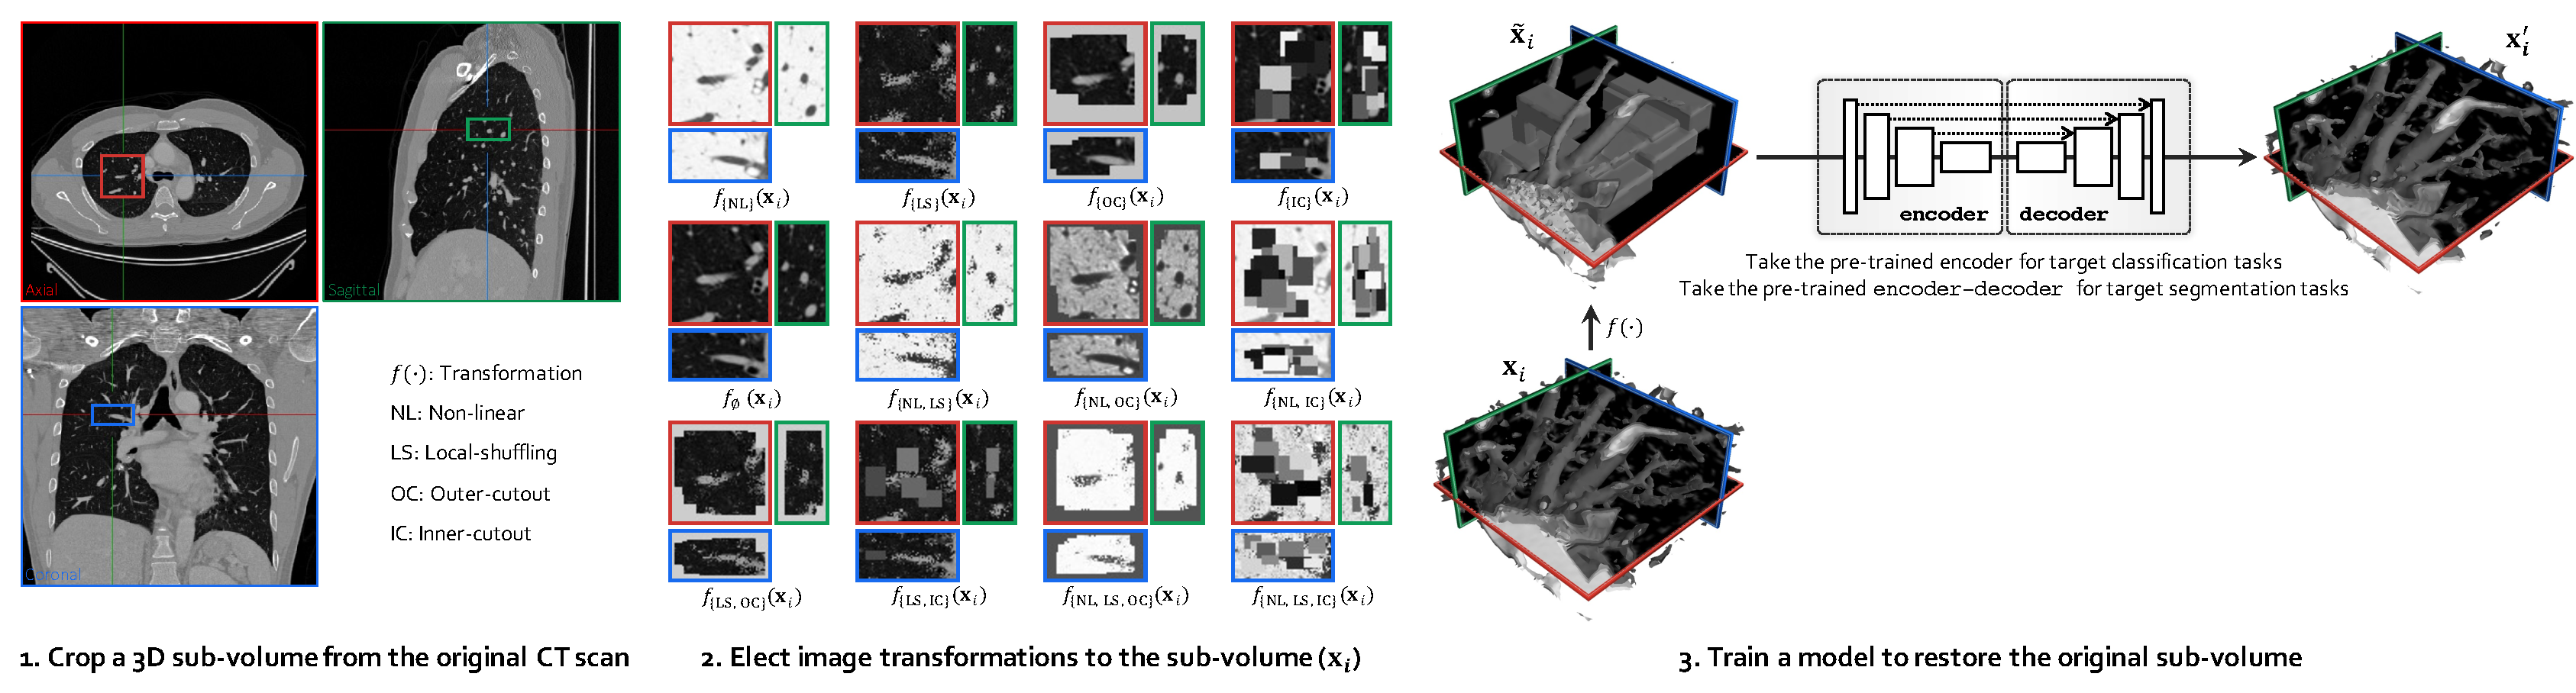
\includegraphics[width=1.0\linewidth]{Figures/CH5/fig_genesis_method.pdf}
\end{center}
\caption[Models Genesis Learn Generic Features by Image Restoration]{
Our self-supervised learning framework aims to learn general-purpose image representation by recovering the original sub-volumes of images from their transformed ones. We first crop arbitrarily-size sub-volume $\textbf{x}_i$ at a random location from an unlabeled CT image. Each sub-volume $\textbf{x}_i$ can undergo at most three out of four transformations: non-linear, local-shuffling, outer-cutout, and inner-cutout, resulting in a transformed sub-volume $\tilde{\textbf{x}}_i$. It should be noted that outer-cutout and inner-cutout are considered mutually exclusive. Therefore, in addition to the four original individual transformations, this process yields eight more transformations, including one identity mapping ($\phi$ meaning none of the four individual transformations is selected) and seven combined transformations. A Model Genesis, an encoder-decoder architecture with skip connections in between, is trained to learn a common image representation by restoring the original sub-volume $\textbf{x}_i$ (as ground truth) from the transformed one $\tilde{\textbf{x}}_i$ (as input), in which the reconstruction loss (MSE) is computed between the model prediction $\textbf{x}_i'$ and ground truth $\textbf{x}_i$. Once trained, the encoder alone can be fine-tuned for target classification tasks; while the encoder and decoder together can be fine-tuned for target segmentation tasks. 
}
\label{ch5:fig:self_supervised_learning_framework}
\end{sidewaysfigure}

% \fillandplacepagenumber
% \end{landscape}
%%%%%%%%%%%%%%%%%%%%%%%%%%%%%%%%%%%%%%%%%%%%



%%%%%%%%%%%%%%%%%%%%%%%%%%%%%%%%%%%%%%%%%%%%
% \begin{landscape}
% \thispagestyle{empty}

\begin{sidewaysfigure}
\begin{center}
\includegraphics[width=0.9\columnwidth]{Figures/CH5/fig_transformations.pdf}
\end{center}
\caption[Illustration of Image Transformations and Learning Perspectives]{
Illustration of the proposed image transformations and their learning perspectives. For simplicity and clarity, we illustrate the transformation on a 2D CT slice, but our Genesis Chest CT is trained directly using 3D sub-volumes, which are transformed in a 3D manner. For ease of understanding, in (a) non-linear transformation, we have displayed an image undergoing different translating functions in Columns 2---7; in (b) local-shuffling, (c) outer-cutout, and (d) inner-cutout transformation, we have illustrated each of the processes step by step in Columns 2---6, where the first and last columns denote the original images and the final transformed images, respectively. In local-shuffling, a different window $\mathbf{W}$ is automatically generated and used in each step. We provide the implementation details in Sec.~\ref{ch5:image_transformation}.
}
\label{ch5:fig:image_transformations}
\end{sidewaysfigure}

% \fillandplacepagenumber
% \end{landscape}
%%%%%%%%%%%%%%%%%%%%%%%%%%%%%%%%%%%%%%%%%%%%


% \section{First Generic Pre-trained 3D Models for Medical Image Analysis}
\section{Approach \& Property}
\label{ch5:method}

The objective of Models Genesis is to learn a common image representation that is transferable and generalizable across diseases, organs, and modalities. 
\figurename~\ref{ch5:fig:self_supervised_learning_framework} depicts our self-supervised learning framework, which enables training 3D models from scratch using unlabeled images, consisting of three steps: (1) cropping sub-volumes from patient CT images, (2) deforming the sub-volumes, and (3) training a model to restore the original sub-volume. In the following sections, we first introduce the denotations of our self-supervised learning framework and then detail each of the training schemes with its learning objectives and perspectives, followed by a summary of the four unique properties of our Models Genesis.

% \subsection{Image restoration proxy task}
\subsection{Learning by Image Restoration}

Given a raw dataset consisting of $N$ patient volumes, theoretically we can crop infinite number of sub-volumes from the dataset. In practice, we randomly generate a subset $\mathcal{X}=\{\mathbf{x_1},\mathbf{x_2},...,\mathbf{x_n}\}$, which includes $n$ number of sub-volumes and then apply image transformation function to these sub-volumes, yielding
\begin{equation}
    \tilde{\mathcal{X}} = f(\mathcal{X}),
\end{equation}
where $\tilde{\mathcal{X}}=\{\mathbf{\tilde{x}_1},\mathbf{\tilde{x}_2},...,\mathbf{\tilde{x}_n}\}$ and $f(\cdot)$ denotes a transformation function. Subsequently, a Model Genesis, being an encoder-decoder network with skip connections in between, will learn to approximate the function $g(\cdot)$ which aims to map the transformed sub-volumes $\tilde{\mathcal{X}}$ back to their original ones $\mathcal{X}$, that is,
\begin{equation}
    g(\tilde{\mathcal{X}}) = \mathcal{X} =  f^{-1}(\tilde{\mathcal{X}}).
\end{equation}

To avoid heavy weight dedicated towers for each proxy task and to maximize parameter sharing in Models Genesis, we consolidate four self-supervised schemes into a single image restoration task, enabling models to learn robust image representation by restoring from various sets of image transformations. Our proposed framework includes four transformations: (1) non-linear, (2) local-shuffling, (3) outer-cutout, and (4) inner-cutout.
Each transformation is independently applied to a sub-volume with a predefined probability, while outer-cutout and inner-cutout are considered mutually exclusive. Consequently, each sub-volume can undergo at most three of the above transformations, resulting in twelve possible transformed sub-volume (see step 2 in~\figurename~\ref{ch5:fig:self_supervised_learning_framework}). For clarity, we further define a {\em training scheme} as the process that (1) transforms sub-volumes using any of the aforementioned transformations, and (2) trains a model to restore the original sub-volumes from the transformed ones. For convenience, we refer to an {\em individual training scheme} as the scheme using one particular individual transformation.
We should emphasize that our ultimate goal is not the task of image restoration \textit{per se}. While restoring images is advocated and investigated as a training scheme for models to learn image representation, the usefulness of the learned representation must be assessed \textit{objectively} based on its generalizability and transferability to various target tasks.


\subsection{Learning from Multiple Perspectives}
\label{ch5:image_transformation}

\textit{1) Learning appearance via non-linear transformation.} We propose a novel self-supervised training scheme based on non-linear translation, with which the model learns to restore the intensity values of an input image transformed with a set of non-linear functions. The rationale is that the absolute intensity values (\ie Hounsfield units) in CT scans or relative intensity values in other imaging modalities convey important information about the underlying structures and organs~\citep{prince2006medical,buzug2011computed,forbes2012human}. Hence, this training scheme enables the model to learn the appearance of the anatomic structures present in the images. In order to keep the appearance of the anatomic structures perceivable, we intentionally retain the non-linear intensity transformation function as \textit{monotonic}, allowing pixels of different values to be assigned with new distinct values. To realize this idea, we use B{\'e}zier Curve~\citep{mortenson1999mathematics}, a smooth and monotonic transformation function, which is generated from two end points ($P_0$ and $P_3$) and two control points ($P_1$ and $P_2$), defined as:
\begin{equation}
    B(t)=(1-t)^3P_0+3(1-t)^2tP_1+3(1-t)t^2P_2+t^3P_3,\ t\in [0,1],
\end{equation}
where $t$ is a fractional value along the length of the line. In \figurename~\ref{ch5:fig:image_transformations}(a), we illustrate the original CT sub-volume (the left-most column) and its transformed ones based on different transformation functions. The corresponding transformation functions are shown in the top row. Notice that, when $P_0 = P_1$ and $P_2 = P_3$ the B{\'e}zier Curve is a linear function (shown in Columns 2, 5). Besides, we set $P_0 = (0,0)$ and $P_3 = (1,1)$ to get an increasing function (shown in Columns 2---4) and the opposite to get a decreasing function (shown in Columns 5---7). The control points are randomly generated for more variances (shown in Columns 3, 4, 6, 7). Before applying the transformation functions, in Genesis CT, we first clip the Hounsfield units values within the range of $[-1000, 1000]$ and then normalize each CT scan to $[0, 1]$.
     
\textit{2) Learning texture via local pixel shuffling.} We propose local pixel shuffling to enrich local variations of a sub-volume without dramatically compromising its global structures, which encourages the model to learn the {\em local} boundaries and textures of objects. To be specific, for each input sub-volume, we randomly select 1,000 windows and then shuffle the pixels inside each window sequentially. Mathematically, let us consider a small window $\mathbf{W}$ with a size of $m\times n$.
The local-shuffling acts on each window and can be formulated as
\begin{equation}
    \tilde{\mathbf{W}}=\mathbf{P}\times\mathbf{W}\times\mathbf{P}',
\end{equation}
where $\tilde{\mathbf{W}}$ is the transformed window, $\mathbf{P}$ and $\mathbf{P}'$ denote permutation metrics with the size of $m\times m$ and $n\times n$, respectively. Pre-multiplying $\mathbf{W}$ with $\mathbf{P}$ permutes the rows of the window $\mathbf{W}$, whereas post-multiplying $\mathbf{W}$ with $\mathbf{P}'$ results in the permutation of the columns of the window $\mathbf{W}$. The size of the local window determines the difficulty of proxy task. In practice, to preserve the global content of the image, we keep the window sizes smaller than the receptive field of the network, so that the network can learn much more robust image representation by ``resetting'' the original pixels positions. Note that our method is quite different from PatchShuffling~\citep{kang2017patchshuffle}, which is a regularization technique to avoid over-fitting. Unlike de-noising~\citep{vincent2010stacked} and in-painting~\citep{pathak2016context,iizuka2017globally}, our local-shuffling transformation does not intend to replace the pixel values with noise, which therefore preserves the identical global distributions to the original sub-volume. 
In addition, local-shuffling within an extent keeps the objects perceivable, as shown in \figurename~\ref{ch5:fig:image_transformations}(b), benefiting the deep neural network in learning \textit{local} invariant image representations, which serves as a complementary perspective with global patch shuffling~\citep{chen2019self}.


\textit{3) Learning context via outer and inner cutouts.} We devise outer-cutout as a new training scheme for self-supervised learning\footnote{I acknowledge Vatsal Sodha, with whom I co-authored~\citet{zhou2019models,zhou2021models}, for implementing the outer cutout learning scheme~\citep{sodha2020self}.}. To realize it, we generate an arbitrary number ($\leq 10$) of windows, with various sizes and aspect ratios, and superimpose them on top of each other, resulting in a single window of a complex shape. When applying this merged window to a sub-volume, we leave the sub-volume region inside the window exposed and mask its surrounding (\ie outer-cutout) with a random number. 
Moreover, to prevent the task from being too difficult or even unsolvable, we extensively search for the optimal size of cutout regions spanning from 0\% to 90\%, incremented by 10\%. In the end, we limit the outer-cutout region to be less than 1/4 of the whole sub-volume.
By restoring the outer-cutouts, the model will learn the {\em global} geometry and spatial layout of organs in medical images via extrapolating within each sub-volume. We have illustrated this process step by step in \figurename~\ref{ch5:fig:image_transformations}(c). The first and last columns denote the original sub-volumes and the final transformed sub-volumes, respectively. 

Our self-supervised learning framework also utilizes inner-cutout as a training scheme, where we mask the inner window regions (\ie inner-cutouts) and leave their surroundings exposed. By restoring the inner-cutouts, the model will learn {\em local} continuities of organs in medical images via interpolating within each sub-volume. Unlike \citet{pathak2016context}, where in-painting is proposed as a proxy task by restoring only the central region of the image, we restore the entire sub-volume as the model output. Examples of inner-cutout are illustrated in \figurename~\ref{ch5:fig:image_transformations}(d). 
Following the suggestion from~\citet{pathak2016context}, the inner-cutout areas are limited to be less than $1/4$ of the whole sub-volume, in order to keep the task reasonably difficult.


% \subsection{Unique properties of Models Genesis}
\subsection{Four Unique Properties}
\label{ch5:approach_property:several_unique_properties}

\begin{enumerate}
    \item \textit{Autodidactic---requiring no manual labeling.} Models Genesis are trained in a self-supervised manner with abundant unlabeled image datasets, demanding {\em zero} expert annotation effort. Consequently, Models Genesis are fundamentally different from traditional (fully) {\em supervised} transfer learning from ImageNet~\citep{bar2015chest,shin2016deep,tajbakhsh2016convolutional}, which offers modest benefits to 3D medical imaging applications as well as that from the existing pre-trained, full-supervised models including I3D~\citep{carreira2017quo}, NiftyNet~\citep{gibson2018niftynet}, and MedicalNet~\citep{chen2019med3d}, which demand a volume of annotation effort to obtain the source models (statistics given in \tablename~\ref{ch5:tab:terminology}). To our best knowledge, this work represents the first effort to establish publicly-available, autodidactic models for 3D medical image analysis.
    
    \item \textit{Robust---learning from multiple perspectives.} Our combined approach trains Models Genesis from multiple perspectives (appearance, texture, context, etc.), leading to more robust models across all target tasks, as evidenced in \figureautorefname~\ref{ch5:fig:combined_vs_individuals}, where our combined approach is compared with our individual schemes. This eclectic approach, incorporating multiple tasks into a single image restoration task, empowers Models Genesis to learn more comprehensive representation. While most self-supervised methods devise isolated training schemes to learn from specific perspectives---learning intensity value via colorization, context information via Jigsaw, orientation via rotation, etc---these methods are reported with mixed results on different tasks, in review papers such as~\citet{goyal2019scaling},~\citet{kolesnikov2019revisiting},~\citet{taleb20203d}, and~\citet{jing2020self}. It is critical as a multitude of state-of-the-art results in the literature show the importance of using compositions of more than one transformations per image~\citep{graham2014fractional,dosovitskiy2015discriminative,wu2020generalization}, which has also been experimentally confirmed in our image restoration task.
    
    \item \textit{Scalable---accommodating many training schemes.} Consolidated into a single image restoration task, our novel self-supervised schemes share the same encoder and decoder during training. Had each task required its own decoder, due to limited memory on GPUs, our framework would have failed to accommodate a large number of self-supervised tasks. By unifying all tasks as a single image restoration task, any favorable transformation can be easily amended into our framework, overcoming the scalability issue associated with multi-task learning~\citep{doersch2017multi,noroozi2018boosting,standley2020tasks,chen2019med3d}, where the network heads are subject to the specific proxy tasks.
    
    \item \textit{Generic---yielding diverse applications.} Models Genesis, trained via a diverse set of self-supervised schemes, learn a general-purpose image representation that can be leveraged for a wide range of target tasks. Specifically, Models Genesis can be utilized to initialize the encoder for the target {\em classification} tasks and to initialize the encoder-decoder for the target {\em segmentation} tasks, while the existing self-supervised approaches are largely focused on providing encoder models only~\citep{jing2020self}. As shown in \tablename~\ref{ch5:tab:top_existing_models}, Models Genesis can be generalized across diseases (\eg nodule, embolism, tumor), organs (\eg lung, liver, brain), and modalities (\eg CT and MRI), a generic behavior that sets us apart from all previous works in the literature where the  representation is learned via a specific self-supervised task, and thus lack generality.
    
\end{enumerate}


\begin{table}[t]
\centering
\footnotesize
\caption[Semantic Distance among Source and Target Datasets]{
    Genesis CT is pre-trained on \textit{only} LUNA~2016 dataset (\ie the source) and then fine-tuned for five distinct medical image applications (\ie the targets). These target tasks are selected such that they show varying levels of semantic distance from the source, in terms of organs, diseases, and modalities, allowing us to investigate the transferability of the pre-trained weights of Genesis CT with respect to the domain distance. The cells checked by \xmark \ denote the properties that are different between the source and target datasets.
}
\label{ch5:tab:distance}
\begin{tabular}{p{0.26\linewidth}P{0.15\linewidth}P{0.15\linewidth}P{0.15\linewidth}P{0.15\linewidth}}
    \hline
    Task & Disease & Organ & Dataset & Modality \\
    \hline
    \texttt{NCC} &  \\
    \texttt{NCS} &  \\
    \texttt{ECC} & \xmark & & \xmark \\
    \texttt{LCS} & \xmark & \xmark & \xmark \\
    \texttt{BMS} & \xmark & \xmark & \xmark & \xmark \\
    \hline
\end{tabular}
\end{table}





\section{Experiment \& Result}
\label{ch5:experiments}


In this section, we begin with an ablation study to compare the combined approach with each individual scheme, concluding that the combined approach tends to achieve more robust results and consistently exceeds any other training schemes. We then take our pre-trained model from the combined approach and present results on five 3D medical applications, comparing them against the state-of-the-art approaches found in recent supervised and self-supervised learning literature.


%%%%%%%%%%%%%%%%%%%%%%%%%%%%%%%%%%%%%%%%%%%%
% \begin{landscape}
% \thispagestyle{empty}

\begin{sidewaysfigure}
\begin{center}
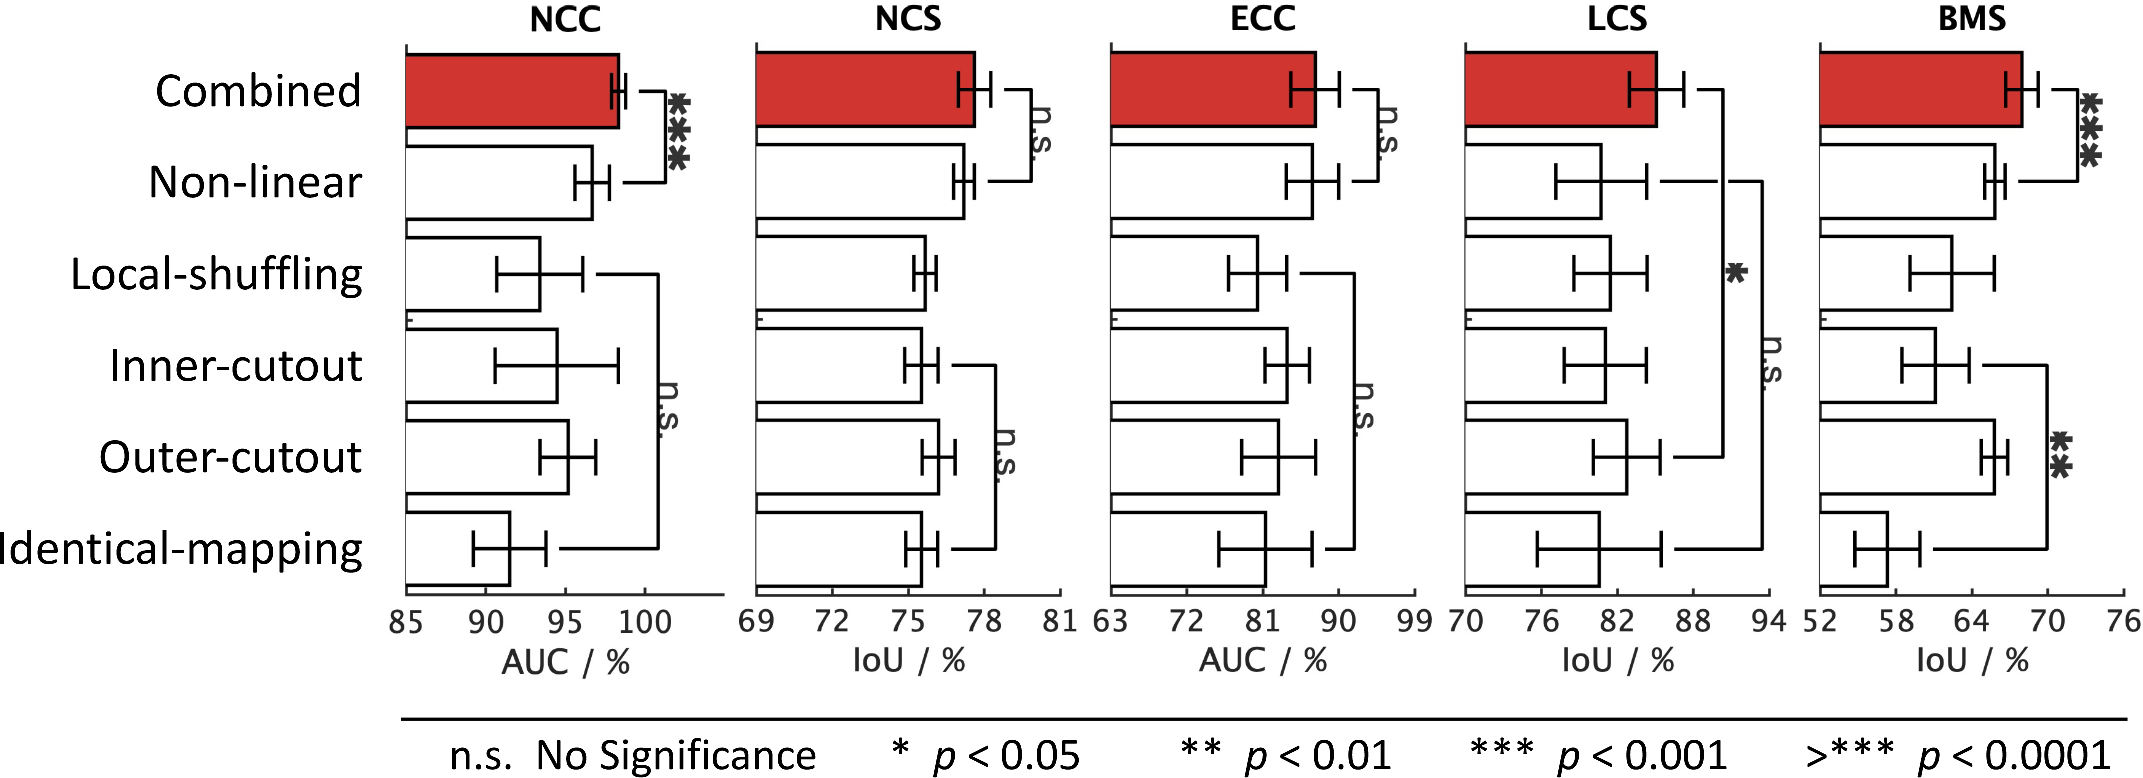
\includegraphics[width=0.9\columnwidth]{Figures/CH5/fig_combined_vs_individuals.pdf}
\end{center}
\caption[The Combined Learning Scheme Exceeds Each Individual]{
Comparing the combined training scheme with each of the proposed individual training schemes, we conduct statistical analyses between the top two training schemes as well as between the bottom two. Although some of the individual training schemes could be favorable for certain target tasks, there is no such clear clue to guarantee that any one of the individual training schemes would consistently offer the best performance on every target task. On the contrary, our combined training scheme consistently achieves the best results across all five target tasks.
}
\label{ch5:fig:combined_vs_individuals}
\end{sidewaysfigure}

% \fillandplacepagenumber
% \end{landscape}
%%%%%%%%%%%%%%%%%%%%%%%%%%%%%%%%%%%%%%%%%%%%

\subsection{The Combined Learning Scheme Exceeds Each Individual}
\label{ch5:individual_combination}


We have devised four individual training schemes by applying each of the transformations (\ie non-linear, local-shuffling, outer-cutout, and inner-cutout) individually to a sub-volume and training the model to restore the original one. We compare each of these training schemes with identical-mapping, which does not involve any image transformation\footnote{I acknowledge Vatsal Sodha, with whom I co-authored~\citet{zhou2019models,zhou2021models}, for comparing the combined learning scheme with each individual.}. In three out of the five target tasks, as shown in Figs.~\ref{ch5:fig:combined_vs_individuals}---\ref{ch5:fig:random_initialization}, the model pre-trained by identical-mapping scheme does not perform as well as random initialization. This undesired representation obtained via identical-mapping suggests that without any image transformation, the model would not benefit much from the proxy image restoration task. On the contrary, nearly all of the individual schemes offer higher target task performances than identical-mapping, demonstrating the significance of the four devised image transformations in learning image representation. 

Although each of the individual schemes has established the capability in learning image representation, its empirical performance varies from task to task. That being said, given a target task, there is no clear winner among the four individual schemes that can always guarantee the highest performance. As a result, we have further devised a combined scheme, which applies transformations to a sub-volume with a predefined probability for each transformation and trains a model to restore the original one. To demonstrate the importance of combining these image transformations together, we examine the combined training scheme against each of the individual ones. \figurename~\ref{ch5:fig:combined_vs_individuals} shows that the combined scheme consistently exceeds any other individual schemes in all five target tasks. We have found that the combination of different transformations is advantageous because, as discussed, we cannot rely on one single training scheme to achieve the most robust and compelling results across multiple target tasks. 
It is our novel representation learning framework based on image restoration that allows integrating various training schemes into a single training scheme. Our qualitative assessment of image restoration quality further indicates that the combined scheme is superior over all four individual schemes in restoring the images that have been undergone multiple transformations. In summary, our combined scheme pre-trains a model from multiple perspectives (appearance, texture, context, etc.), empowering models to learn a more comprehensive representation, thereby leading to more robust target models. Based on the above ablation studies, in the following sections, we refer the models pre-trained by the combined scheme to Models Genesis and, in particular, refer the model pre-trained on LUNA~2016 dataset to Genesis Chest CT.


%%%%%%%%%%%%%%%%%%%%%%%%%%%%%%%%%%%%%%%%%%%%
% \begin{landscape}
% \thispagestyle{empty}

\begin{sidewaysfigure}
\begin{center}
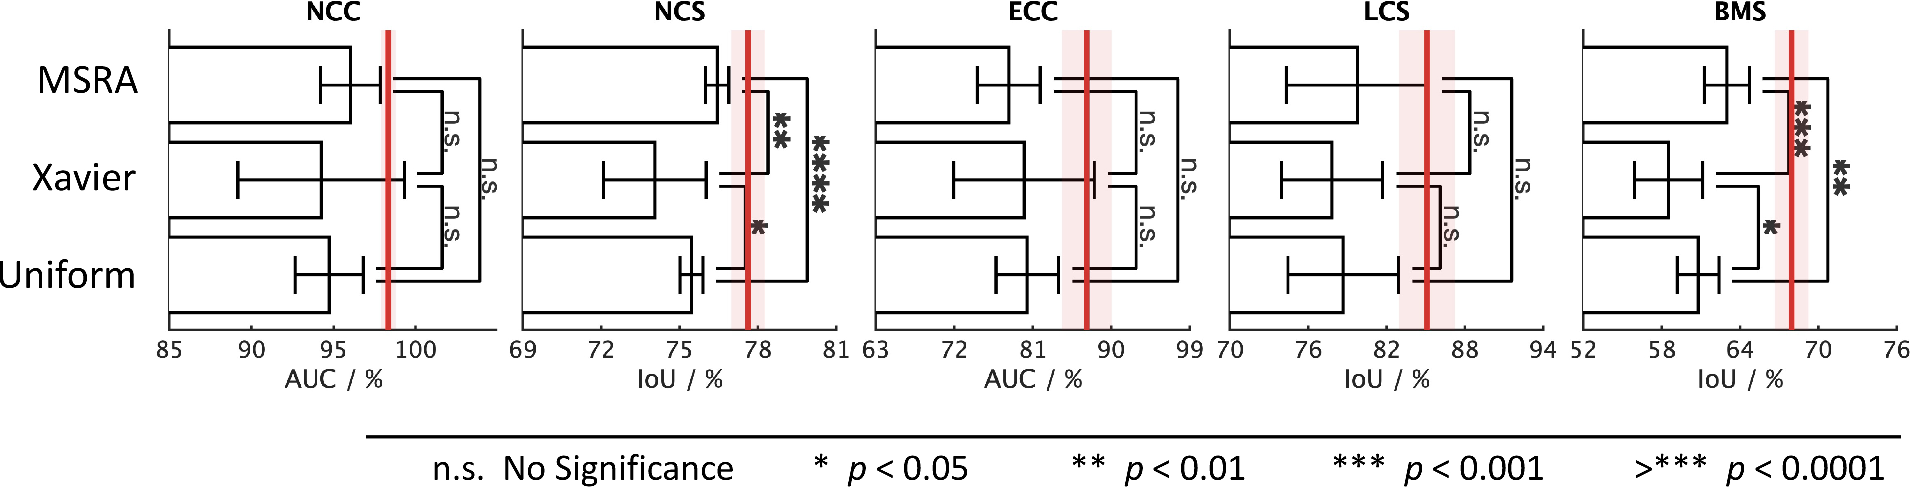
\includegraphics[width=0.9\columnwidth]{Figures/CH5/fig_among_scratch.pdf}
\end{center}
\caption[Models Genesis Outperform Learning from Scratch]{
Models Genesis, as presented with the red vertical lines, achieve higher and more stable performance compared with three popular types of random initialization methods, including MSRA, Xavier, and Uniform. Among three out of the five applications, three different types of random distribution reveal no significant difference with respect to each other.
}
\label{ch5:fig:random_initialization}
\end{sidewaysfigure}

% \fillandplacepagenumber
% \end{landscape}
%%%%%%%%%%%%%%%%%%%%%%%%%%%%%%%%%%%%%%%%%%%%

%%%%%%%%%%%%%%%%%%%%%%%%%%%%%%%%%%%%%%%%%%%%
% \begin{landscape}
% \thispagestyle{empty}

\begin{sidewaysfigure}
\begin{center}
\includegraphics[width=1.0\columnwidth]{Figures/CH5/fig_learning_curve.pdf}
\end{center}
\caption[Models Genesis Enable Better Optimization than Learning from Scratch]{
Models Genesis enable better optimization than learning from scratch, evident by the learning curves for the target tasks of reducing false positives in detecting lung nodules (\texttt{NCC}) and pulmonary embolism (\texttt{ECC}) as well as segmenting lung nodule (\texttt{NCS}), liver (\texttt{LCS}), and brain tumor (\texttt{BMS}). We have plotted the validation performance averaged by ten trials for each application, in which accuracy and dice-coefficient scores are reported for classification and segmentation tasks, respectively. As seen, initializing with our pre-trained Models Genesis demonstrates benefits in the convergence speed.
}
\label{ch5:fig:learning_curve}
\end{sidewaysfigure}

% \fillandplacepagenumber
% \end{landscape}
%%%%%%%%%%%%%%%%%%%%%%%%%%%%%%%%%%%%%%%%%%%%

\subsection{Models Genesis Outperform Learning from Scratch}
\label{ch5:surpass_scratch}


Transfer learning accelerates training and boosts performance, only if the image representation learned from the original (proxy) task is general and transferable to target tasks. Fine-tuning models trained on ImageNet has been a great success story in 2D~\citep{bar2015chest,tajbakhsh2016convolutional,shin2016deep}, but for 3D representation learning, there is no such a massive labeled dataset like ImageNet. As a result, it is still common practice to train 3D model from scratch in 3D medical imaging.
Therefore, to establish the 3D baselines, we have trained 3D models with three representative random initialization methods\footnote{I thank Pengfei Zhang for comparing Xavier/Glorot and He normal (MSRA) initialization methods with our Models Genesis.}, including naive uniform initialization, Xavier/Glorot initialization proposed by~\citet{glorot2010understanding}, and He normal (MSRA) initialization proposed by~\citet{he2015delving}. 
When comparing deep model initialization by transfer learning and by controlling mathematical distribution, the former learns more sophisticated image representation but suffers from a domain gap, whereas the latter is task independent yet provides relatively less benefit than the former. The hypothesis underneath transfer learning is that transferring deep features across visual tasks can obtain a semantically more powerful representation, compared with simply initializing weights using different distributions.
From our comprehensive experiments in~\figurename~\ref{ch5:fig:random_initialization}, we have observed the following:
\begin{itemize}
    \item Within each method, random initialization of weights has shown large variance in results of ten trials; it is in large part due to the difficulty of adequately initializing these networks from scratch. A small miscalibration of the initial weights can lead to vanishing or exploding gradients, as well as poor convergence properties. 
    \item In three out of the five 3D medical applications, the results reveal no significant difference among these random initialization methods. Although randomly initializing weights can vary by the behaviors on different applications, He normal (MSRA), in which the weights are initialized with a specific ReLU-aware initialization, generally works the most reliably among all five target tasks.
    \item On the other hand, initialization with our pre-trained Genesis Chest CT stabilizes the overall performance and, more importantly, elevates the average performance over all three random initialization methods by a large margin. Our statistical analysis shows that the performance gain is significant for all the target tasks under study. This suggests that, owing to the representation learning scheme, our initial weights provide a better starting point than the ones generated under particular statistical distributions, while being over 13\% faster (see \figurename~\ref{ch5:fig:learning_curve}). This observation has also been widely obtained in 2D model initialization~\citep{tajbakhsh2016convolutional,shin2016deep,rawat2017deep,zhou2017fine,voulodimos2018deep}.
\end{itemize}

Altogether, in contrast to 3D scratch models, we believe Models Genesis can potentially serve as a primary source of transfer learning for 3D medical imaging applications. Besides contrasting with the three random initialization methods, we further examine our Models Genesis against the existing pre-trained 3D models in the coming section.



%%%%%%%%%%%%%%%%%%%%%%%%%%%%%%%%%%%%%%%%%%%%
% \begin{landscape}
% \thispagestyle{empty}

\begin{sidewaystable}
\begin{threeparttable}[t]
\begin{center}
\footnotesize
\caption[Models Genesis Surpass Existing Pre-trained 3D Models]{
Models Genesis surpass existing pre-trained 3D models. We evaluate AUC score for classification tasks and IoU score for segmentation tasks. All of the results, including the mean and standard deviation (mean$\pm$s.d.) across ten trials. For every target task, we have further performed independent two sample $t$-test between the best (bolded) vs. others and highlighted boxes in blue when they are not statistically significantly different at $p=0.05$ level.
% Our Models Genesis lead the best or comparable performance on five distinct medical target tasks over six self-supervised learning approaches (revised in 3D) and three competing publicly available (fully) supervised pre-trained 3D models. For ease of comparison, we evaluate AUC score for the two classification tasks (\ie \texttt{NCC} and \texttt{ECC}) and IoU score for the three segmentation tasks (\ie \texttt{NCS}, \texttt{LCS}, and \texttt{BMS}). All of the results, including the mean and standard deviation (mean$\pm$s.d.) across ten trials, reported in the table are evaluated using our dataset splitting, elaborated in~Appendix~\ref{ap1}. For every target task, we have further performed independent two sample $t$-test between the best (bolded) vs. others and highlighted boxes in blue when they are not statistically significantly different at $p=0.05$ level.
}
\label{ch5:tab:top_existing_models}
\begin{tabular}{p{0.14\linewidth}p{0.2\linewidth}P{0.1\linewidth}P{0.1\linewidth}P{0.1\linewidth}P{0.1\linewidth}P{0.1\linewidth}}
    \hline
    \multirow{2}{*}{Pre-training} & \multirow{2}{*}{Approach} & \multicolumn{5}{c}{Target tasks} \\
    \cline{3-7}
     & & \texttt{NCC} (\%) & \texttt{NCS} (\%) & \texttt{ECC} (\%) & \texttt{LCS} (\%) & \texttt{BMS} (\%) \\
    \hline
    \multirow{3}{*}{No} & Random with Uniform Init & 94.74$\pm$1.97 & 75.48$\pm$0.43 & 80.36$\pm$3.58 & 78.68$\pm$4.23 & 60.79$\pm$1.60 \\
     & Random with Xavier Init & 94.25$\pm$5.07 & 74.05$\pm$1.97 & 79.99$\pm$8.06 & 77.82$\pm$3.87 & 58.52$\pm$2.61 \\
     & Random with MSRA Init & 96.03$\pm$1.82 & 76.44$\pm$0.45 & 78.24$\pm$3.60 & 79.76$\pm$5.43 & 63.00$\pm$1.73 \\
    \hline
    \multirow{3}{*}{(Fully) supervised} & I3D & \cellcolor{iblue!30}98.26$\pm$0.27 & 71.58$\pm$0.55 & 80.55$\pm$1.11 & 70.65$\pm$4.26 & \cellcolor{iblue!30}67.83$\pm$0.75 \\
     & NiftyNet & 94.14$\pm$4.57 & 52.98$\pm$2.05 & 77.33$\pm$8.05 & 83.23$\pm$1.05 & 60.78$\pm$1.60  \\
     & MedicalNet & 95.80$\pm$0.49 & 75.68$\pm$0.32 & \cellcolor{iblue!30}86.43$\pm$1.44 & \cellcolor{iblue!30}\textbf{85.52$\pm$0.58} & 66.09$\pm$1.35 \\
    \hline
    \multirow{7}{*}{Self-supervised} & De-noising & 95.92$\pm$1.83 & 73.99$\pm$0.62 & \cellcolor{iblue!30}85.14$\pm$3.02 & 84.36$\pm$0.96 & 57.83$\pm$1.57 \\
     & In-painting & 91.46$\pm$2.97 & 76.02$\pm$0.55 & 79.79$\pm$3.55 & 81.36$\pm$4.83 & 61.38$\pm$3.84 \\
     & Jigsaw & 95.47$\pm$1.24 & 70.90$\pm$1.55 & 81.79$\pm$1.04 & 82.04$\pm$1.26 & 63.33$\pm$1.11 \\
     & DeepCluster & 97.22$\pm$0.55 & 74.95$\pm$0.46 & 84.82$\pm$0.62 & 82.66$\pm$1.00 & 65.96$\pm$0.85 \\
     & Patch shuffling & 91.93$\pm$2.32 & 75.74$\pm$0.51 & 82.15$\pm$3.30 & 82.82$\pm$2.35 & 52.95$\pm$6.92 \\
     & Rubik’s Cube & 96.24$\pm$1.27 & 72.87$\pm$0.16 & 80.49$\pm$4.64 & 75.59$\pm$0.20 & 62.75$\pm$1.93 \\
     & Genesis Chest CT (ours) & \cellcolor{iblue!30}\textbf{98.34$\pm$0.44} & \cellcolor{iblue!30}\textbf{77.62$\pm$0.64} & \cellcolor{iblue!30}\textbf{87.20$\pm$2.87} & \cellcolor{iblue!30}85.10$\pm$2.15 & \cellcolor{iblue!30}\textbf{67.96$\pm$1.29} \\
    \hline
    \end{tabular}
    \begin{tablenotes}
        \item 
    \end{tablenotes}
\end{center}
\end{threeparttable}
\end{sidewaystable}
% \fillandplacepagenumber
% \end{landscape}
%%%%%%%%%%%%%%%%%%%%%%%%%%%%%%%%%%%%%%%%%%%%



\subsection{Models Genesis Surpass Existing Pre-trained 3D Models}
\label{ch5:public_3d_model}

We have evaluated our Models Genesis with existing publicly available pre-trained 3D models on five distinct medical target tasks\footnote{I thank Zuwei Guo for implementing Rubik's Cube~\citep{zhuang2019self} and the 3D version of Jigsaw~\citep{noroozi2016unsupervised} and DeepCluster~\citep{caron2018deep}; Jiaxuan Pang for comparing I3D~\citep{carreira2017quo} with our Models Genesis; Fatemeh Haghighi and Mohammad Reza Hosseinzadeh Taher for implementing the 3D version of in-painting~\citep{pathak2016context}, patch-shuffling~\citep{chen2019self}, and working with Zuwei Guo in evaluating the performance of MedicalNet~\citep{chen2019med3d}; Md Mahfuzur Rahman Siddiquee for examining NiftyNet~\citep{gibson2018niftynet} with our Models Genesis.}. As shown in \tablename~\ref{ch5:tab:top_existing_models}, Genesis Chest CT noticeably contrasts with any other existing 3D models, which have been pre-trained by full supervision. Note that, in the liver segmentation task (\texttt{LCS}), Genesis Chest CT is slightly outperformed by MedicalNet because of the benefit that MedicalNet gained from its (fully) supervised pre-training  on the LiTS dataset directly. Further statistical tests reveal that Genesis Chest CT still yields comparable performance with MedicalNet at $p=0.05$ level. For the rest four target tasks, Genesis Chest CT achieves superior performance against all its counterparts by a large margin, demonstrating the effectiveness and transferability of the learned features of Models Genesis, which are beneficial for both classification and segmentation tasks. 

More importantly, although Genesis Chest CT is pre-trained on Chest CT only, it can generalize to different organs, diseases, datasets, and even modalities. For instance, the target task of pulmonary embolism false positive reduction is performed in Contrast-Enhanced CT scans that can appear differently from the proxy tasks in normal CT scans; yet, Genesis Chest CT achieves a remarkable improvement over training from scratch, increasing the AUC by 7 points. Moreover, Genesis Chest CT continues to yield a significant IoU gain in liver segmentation even though the proxy task and target task are significantly different in both, diseases affecting the organs (lung vs.~liver) and the dataset itself (LUNA~2016 vs.~LiTS~2017). We have further examined Genesis Chest CT and other existing pre-trained models using MRI Flair images, which represent the widest domain distance between the proxy and target tasks. As reported in \tablename~\ref{ch5:tab:top_existing_models} (\texttt{BMS}), Genesis Chest CT yields nearly a 5-point improvement in comparison with random initialization. The increased performance on the MRI imaging task is a particularly strong demonstration of the transfer learning capabilities of our Genesis Chest CT. 
% To further investigate the behavior of Genesis Chest CT when encountering medical images from different modalities, we have provided extensive visualization in \figurename~\ref{ch5:fig:xray_across_restoration}, including example images from CT, X-ray, Ultrasound, and MRI modalities.

Considering the model footprint, our Models Genesis take the basic 3D U-Net as the backbone, carrying much fewer parameters than the existing open-source pre-trained 3D models. For example, we have adopted MedicalNet with resnet-101 as the backbone, which offers the highest performance based on \citet{chen2019med3d} but comprises of 85.75M parameters; the pre-trained I3D~\citep{carreira2017quo} contains 25.35M parameters in the encoder; \iffalse and 134.65M when adding a decoder for segmentation;\fi the pre-trained NiftyNet uses Dense V-Networks~\citep{gibson2018automatic} as backbone, comprising of only 2.60M parameters, but it does not perform as well as its counterparts in all five target tasks. Taken together, these results indicate that our Models Genesis, with only 16.32M parameters, surpass all existing pre-trained 3D models in terms of generalizability, transferability, and parameter efficiency.


%%%%%%%%%%%%%%%%%%%%%%%%%%%%%%%%%%%%%%%%%%%%
% \begin{landscape}
% \thispagestyle{empty}

\begin{sidewaysfigure}
\begin{center}
\includegraphics[width=1.0\columnwidth]{Figures/CH5/fig_annotation_cost.pdf}
\caption[Models Genesis Reduce Annotation Efforts by at Least 30\%]{
Initializing with our Models Genesis, the annotation cost can be reduced by 30\%, 50\%, 57\%, 84\%, and 44\% for target tasks \texttt{NCC}, \texttt{NCS}, \texttt{ECC}, \texttt{LCS}, and \texttt{BMS}, respectively. With decreasing amounts of labeled data, Models Genesis (red) retain a much higher performance on all five target tasks, whereas learning from scratch (grey) fails to generalize. Note that the horizontal red and gray lines refer to the performances that can eventually be achieved by Models Genesis and learning from scratch, respectively, when using the entire dataset.
}
\label{ch5:fig:annotation_cost}
\end{center}
\end{sidewaysfigure}

% \fillandplacepagenumber
% \end{landscape}
%%%%%%%%%%%%%%%%%%%%%%%%%%%%%%%%%%%%%%%%%%%%


\subsection{Models Genesis Reduce Annotation Efforts by at Least 30\%}
\label{ch5:annotation_effort}

While critics often stress the need for sufficiently large amounts of labeled data to train a deep model, transfer learning leverages the knowledge about medical images already learned by pre-trained models and therefore requires considerably fewer annotated data and training iterations than learning from scratch. We have simulated the scenarios of using a handful of labeled data, which allows investigating the power of our Models Genesis in transfer learning. \figurename~\ref{ch5:fig:annotation_cost} displays the results of training with a partial dataset, demonstrating that fine-tuning Models Genesis saturates quickly on the target tasks since it can achieve similar performance compared with the full dataset training. 
Specifically, the performance of learning 3D models from scratch with entire datasets can be approximated using Models Genesis with only 50\%, 5\%, 30\%, 5\%, and 30\% of datasets for \texttt{NCC}, \texttt{NCS}, \texttt{ECC}, \texttt{LCS}, and \texttt{BMS}, respectively. 
This shows that our Models Genesis can mitigate the lack of labeled images, resulting in a more annotation efficient deep learning in the end. 

Furthermore, the performance gap between fine-tuning and learning from scratch is significant and steady over training models with each partial data point. For the lung nodule false positive reduction target task (\texttt{NCC} in~\figurename~\ref{ch5:fig:annotation_cost}), using only 49\% training data, Models Genesis equal the performance of 70\% training data learning from scratch. Therefore, about 30\% of the annotation cost associated with learning from scratch in \texttt{NCC} is recovered by initializing with Models Genesis. For the lung nodule segmentation target task (\texttt{NCS} in~\figurename~\ref{ch5:fig:annotation_cost}), with 5\% training data, Models Genesis can achieve the performance equivalent to learning from scratch using 10\% training data. Based on this analysis, the cost of annotation in \texttt{NCS} can be reduced by half using Models Genesis compared with learning from scratch. For the pulmonary embolism false positive reduction target task (\texttt{ECC}),~\figurename~\ref{ch5:fig:annotation_cost} suggests that with only 30\% training samples, Models Genesis achieve performance equivalent to learning from scratch using 70\% training samples. Therefore, nearly 57\% of the labeling cost associated with the use of learning from scratch for \texttt{ECC} could be recovered with our Models Genesis. For the liver segmentation target task (\texttt{LCS}) in~\figurename~\ref{ch5:fig:annotation_cost}, using 8\% training data, Models Genesis equal the performance of learning from scratch using 50\% training samples. Therefore, about 84\% of the annotation cost associated with learning from scratch in \texttt{LCS} is recovered by initializing with Models Genesis. For the brain tumor segmentation target task (\texttt{BMS}) in~\figurename~\ref{ch5:fig:annotation_cost}, with less than 28\% training data, Models Genesis achieve the performance equivalent to learning from scratch using 50\% training data. Therefore, nearly 44\% annotation efforts can be reduced using Models Genesis compared with learning from scratch. Overall, at least 30\% annotation efforts have been reduced by Models Genesis, in comparison with learning a 3D model from scratch in five target tasks. With such annotation-efficient 3D transfer learning paradigm, computer-aided diagnosis of rare diseases or rapid response to global pandemics, which are severely underrepresented owing to the difficulty of collecting a sizeable amount labeled data, could be eventually actualized.

%%%%%%%%%%%%%%%%%%%%%%%%%%%%%%%%%%%%%%%%%%%%
% \begin{landscape}
% \thispagestyle{empty}

\begin{sidewaysfigure}
\centering
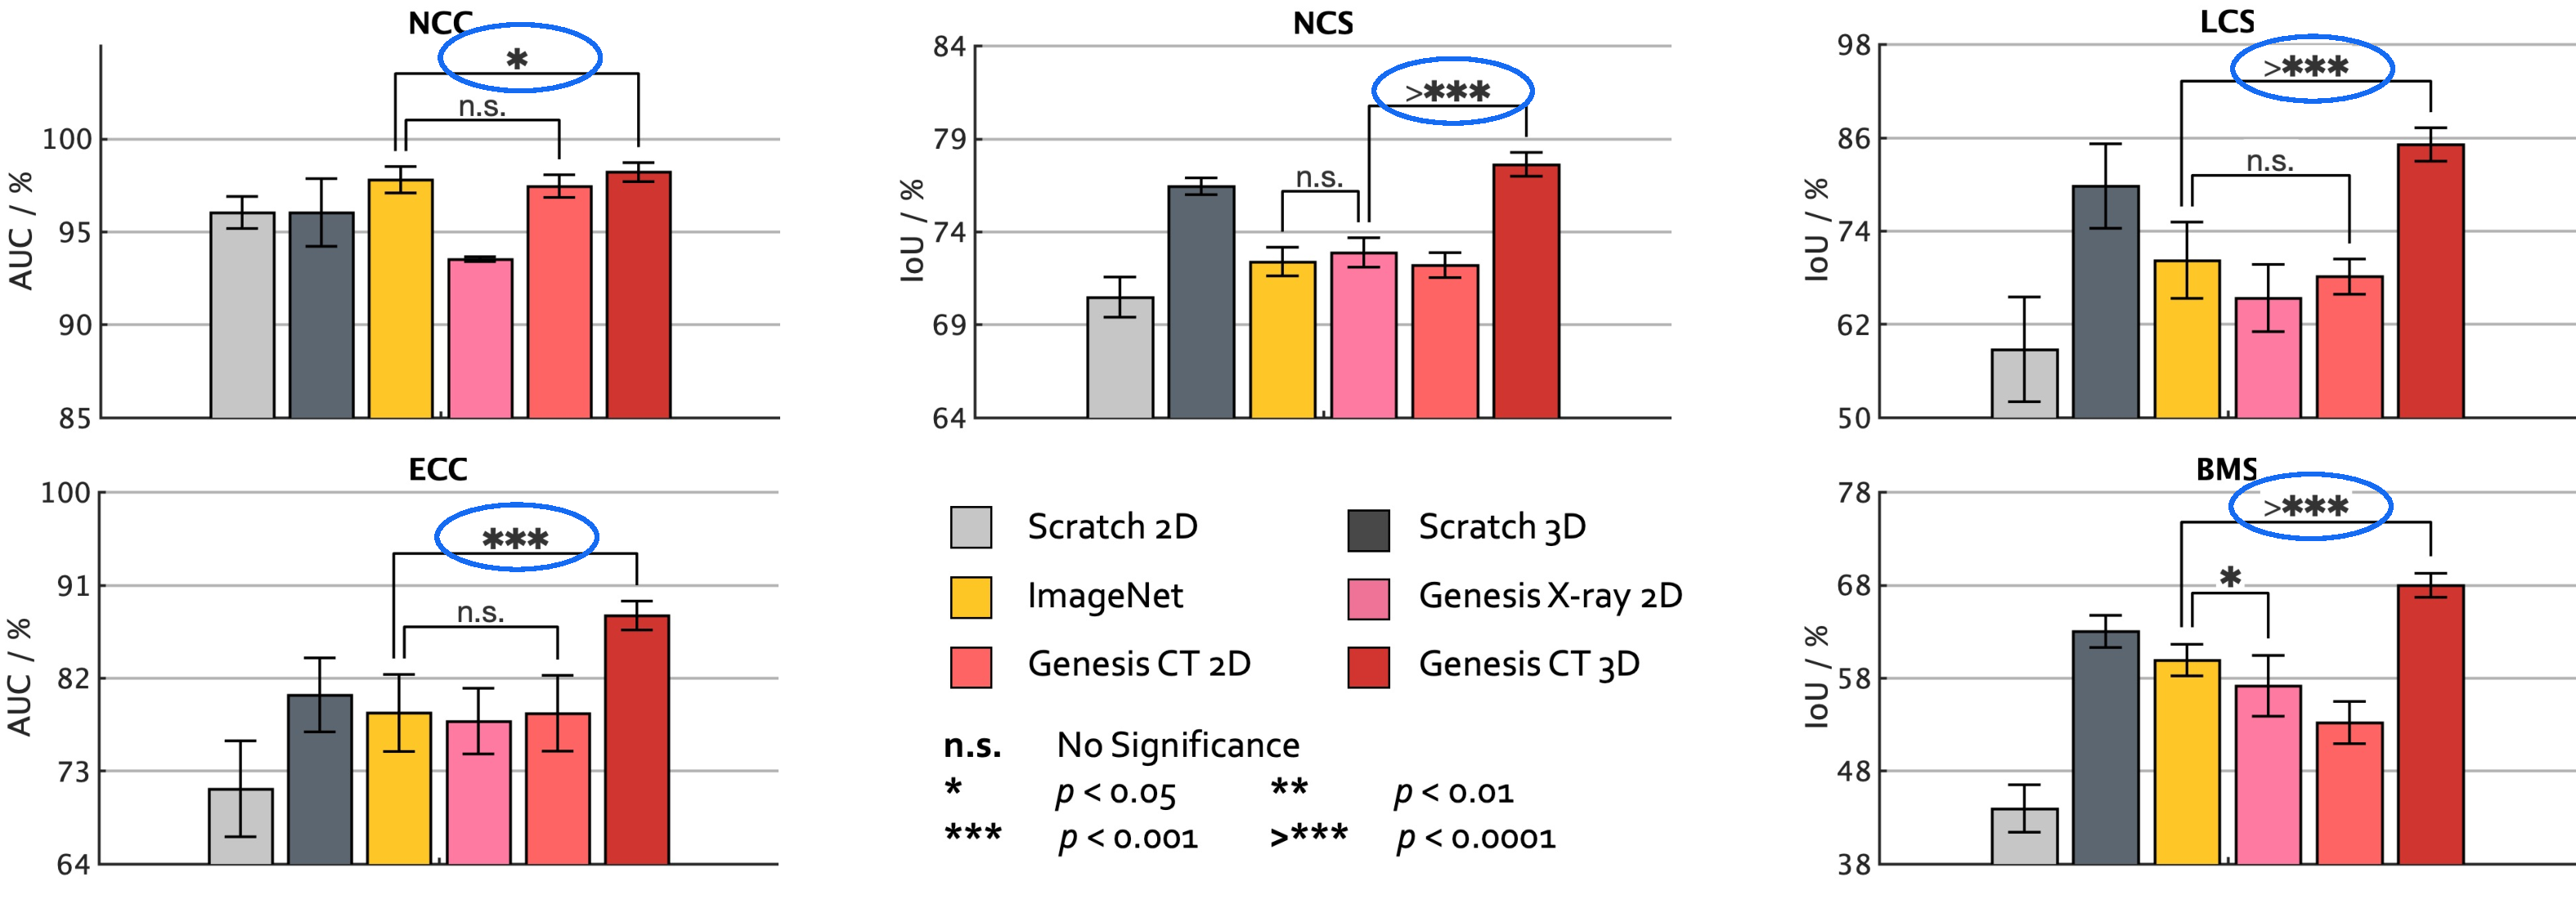
\includegraphics[width=1.0\columnwidth]{Figures/CH5/fig_3d_vs_2d.pdf}
\caption[Models Genesis Top Any 2D Approaches]{
When solving problems in volumetric medical modalities, such as CT and MRI images, 3D \textit{volume-based} approaches consistently offer superior performance than 2D \textit{slice-based} approaches empowered by transfer learning. We conduct statistical analyses (circled in blue) between the highest performance achieved by 3D and 2D solutions. Training 3D models from scratch does not necessarily outperform their 2D counterparts (see \texttt{NCC}). However, training the same 3D models from Genesis Chest CT outperforms all their 2D counterparts, including fine-tuning Models ImageNet as well as fine-tuning our Genesis Chest X-ray and Genesis Chest CT 2D. It confirms the effectiveness of Genesis Chest CT in unlocking the power of 3D models. In addition, we have also provided statistical analyses between the highest and the second highest performances achieved by 2D models, finding that Models Genesis (2D) offer equivalent performances (n.s.) to Models ImageNet in four out of the five applications.
}
\label{ch5:fig:2D_3D_target_tasks}
\end{sidewaysfigure}

% \fillandplacepagenumber
% \end{landscape}
%%%%%%%%%%%%%%%%%%%%%%%%%%%%%%%%%%%%%%%%%%%%


\begin{table}[t]
\centering
\footnotesize
\caption[Models Genesis Top Any 2D/2.5D Approaches]{
Our 3D approach, initialized by Models Genesis, significantly elevates the classification performance compared with 2.5D and 2D approaches in reducing lung nodule and pulmonary embolism false positives. The entries in bold highlight the best results achieved by different approaches. For the 2D slice-based approach, we extract input consisting of three adjacent axial views of the lung nodule or pulmonary embolism and some of their surroundings. For the 2.5D orthogonal approach, each input is composed of an axial, coronal, and sagittal slice and centered at a lung nodule or pulmonary embolism candidate.
}
\label{ch5:tab:3d_2.5d_2d}
\begin{tabular}{p{0.35\linewidth}P{0.18\linewidth}P{0.18\linewidth}P{0.18\linewidth}}
    \hline
    Task: \texttt{NCC} & Random & ImageNet & Genesis \\
    \hline
    2D slice-based input & 96.03$\pm$0.86 & \textbf{97.79$\pm$0.71} & 97.45$\pm$0.61 \\
    2.5D orthogonal input & 95.76$\pm$1.05 & \textbf{97.24$\pm$1.01} & 97.07$\pm$0.92 \\
    3D volume-based input & 96.03$\pm$1.82 & n/a & \textbf{98.34$\pm$0.44} \\
    \hline
    \hline
    Task: \texttt{ECC} & Random & ImageNet & Genesis \\
    \hline
    2D slice-based input & 60.33$\pm$8.61 & 62.57$\pm$8.04 & \textbf{62.84$\pm$8.78} \\
    2.5D orthogonal input & 71.27$\pm$4.64 & \textbf{78.61$\pm$3.73} & 78.58$\pm$3.67 \\
    3D volume-based input & 80.36$\pm$3.58 & n/a & \textbf{88.04$\pm$1.40} \\
    \hline
    \end{tabular}
\end{table}

\subsection{Models Genesis Top Any 2D/2.5D Approaches}
\label{ch5:models_genesis_top_2D}

We have thus far presented the power of 3D models in processing volumetric data, in particular, with limited annotation. Besides adopting 3D models, another common strategy to handle limited data in volumetric medical imaging is to reformat 3D data into a 2D image representation followed by fine-tuning pre-trained Models ImageNet~\citep{shin2016deep,tajbakhsh2016convolutional}. This approach increases the training examples by order of magnitude, but it sacrifices the 3D context. It is interesting to note how Genesis Chest CT compares with this \textit{de facto} standard in 2D. We have thus implemented two different methods to reformat 3D data into 2D input\footnote{I thank Jae Y. Shin for organizing and pre-processing the PE dataset.}: the regular 2D representation obtained by extracting adjacent axial slices~\citep{ben2016fully,sun2017multiphase}, and the 2.5D representation~\citep{prasoon2013deep,roth2014new,roth2015improving} composed of axial, coronal, and sagittal slices from volumetric data. Both of these 2D approaches seek to use 2D representation to emulate something three dimensional, in order to fit the paradigm of fine-tuning Models ImageNet. 
In the inference, classification and segmentation tasks are evaluated differently in 2D: for classification, the model predicts labels of slices extracted from the center locations because other slices are not guaranteed to include objects; for segmentation, the model predicts segmentation mask slice by slice and form the 3D segmentation volume by simply stacking the 2D segmentation maps.


\figurename~\ref{ch5:fig:2D_3D_target_tasks} exposes the comparison between 3D and 2D models on five 3D target tasks. Additionally, \tablename~\ref{ch5:tab:3d_2.5d_2d} compares 2D slice-based, 2.5D orthogonal, and 3D volume-based approaches on lung nodule and pulmonary embolism false positive reduction tasks. As evidenced by our statistical analyses, the 3D models trained from Genesis Chest CT achieve significantly higher average performance and lower standard deviation than 2D models fine-tuned from ImageNet using either 2D or 2.5D image representation. Nonetheless, the same conclusion does not apply to the models trained from scratch---3D scratch models are outperformed by 2D models in one out of the five target tasks (\ie \texttt{NCC} in \figurename~\ref{ch5:fig:2D_3D_target_tasks} and \tablename~\ref{ch5:tab:3d_2.5d_2d}) and also exhibit an undesirably larger standard deviation. We attribute the mixed results of 3D scratch models to the larger number of model parameters and limited sample size in the target tasks, which together impede the full utilization of 3D context. In fact, the undesirable performance of the 3D scratch models highlights the effectiveness of Genesis Chest CT, which unlocks the power of 3D models for medical imaging. To summarize, we believe that 3D problems in medical imaging should be solved in 3D directly.


\section{Discussion \& Conclusion}
\label{ch5:discussion}

%%moved to here
\subsection{Do We Still Need a Medical ImageNet?}
\label{ch5:medical_imagenet}

In computer vision, at the time this chapter is written, no self-supervised learning method outperforms fine-tuning models pre-trained on ImageNet~\citep{jing2020self,chen2019self,kolesnikov2019revisiting,zhou2019models,hendrycks2019using,zhang2019aet,caron2019unsupervised}. Therefore, it may seem surprising to observe from our results in \tablename~\ref{ch5:tab:top_existing_models} that (fully) supervised representation learning methods do not necessarily offer higher performances in some 3D target tasks than self-supervised representation learning methods. We ascribe this phenomenon to the limited amount of supervision used in their pre-training (90 cases for NiftyNet~\citep{gibson2018niftynet} and 1,638 cases for MedicalNet~\citep{chen2019med3d}) or the domain distance (from videos to CT/MRI for I3D~\citep{carreira2017quo}). Evidenced by a prior study~\citep{sun2017revisiting} on ImageNet pre-training, large amount of supervision is required to foster a generic, comprehensive image representation. Back in 2009, when ImageNet had not been established, it was challenging to empower a deep model with generic image representation using a small or even medium size of labeled data, the same situation, we believe, that presents in 3D medical image analysis today. Therefore, despite the outstanding performance of Models Genesis, there is no doubt that a large, strongly annotated dataset for medical image analysis, like ImageNet~\citep{deng2009imagenet} for computer vision, is still highly demanded. One of our goals for developing Models Genesis is to help create such a medical ImageNet. Based on a small set of expert annotations, models fine-tuned from Models Genesis will be able to help quickly generate initial rough annotations of unlabeled images for expert review, thus reducing the annotation efforts and accelerating the creation of a large, strongly annotated, medical ImageNet. In summary, Models Genesis are not designed to replace such a large, strongly annotated dataset for medical image analysis, as ImageNet for computer vision, but rather to help create one.



\subsection{Same-domain or Cross-domain Transfer Learning?}
\label{ch5:same_cross_modality}

Same-domain transfer learning is always preferred whenever possible because a relatively smaller domain gap makes the learned image representation more beneficial for target tasks. Even the most recent self-supervised learning approaches in medical imaging were solely evaluated within the same dataset, such as~\citet{chen2019self,tajbakhsh2019surrogate,zhu2020rubik}. Same-domain transfer learning strikes as a preferred choice in terms of performance; however, most of the existing medical datasets, with less than hundred cases, are usually too small for deep models to learn reliable image representation. Therefore, for our future work, we plan to combine the publicly available datasets from similar domains together to train modality-oriented models, including Genesis CT, Genesis MRI, Genesis X-ray, and Genesis Ultrasound, as well as organ-oriented models, including Genesis Brain, Genesis Lung, Genesis Heart, and Genesis Liver. 

Cross-domain transfer learning in medical imaging is the Holy Grail. Retrieving a large number of unlabeled images from a PACS system requires an IRB approval, often a long process; the retrieved images must be de-identified; organizing the de-identified images in a way suitable for deep learning is tedious and laborious. Therefore, large quantities of unlabeled datasets may not be readily available to many target domains. Evidenced by our results in \tablename~\ref{ch5:tab:top_existing_models} (\texttt{BMS}), Models Genesis have a great potential for cross-domain transfer learning; particularly, our distortion-based approaches (such as non-linear and local-shuffling) take advantage of relative intensity values (in all modalities) to learn shapes and appearances of various organs. Therefore, as our future work, we will be focusing on methods that generalize well across domains. 


\subsection{Is Any Data Augmentation Suitable as a Transformation?} 
\label{ch5:choice_transformations}

We propose a self-supervised learning framework to learn image representation by discriminating and restoring images undergoing different transformations. One might argue that our image transformations can be interchangeable with existing data augmentation techniques~\citep{gan2015learning,wong2016understanding,perez2017effectiveness,shorten2019survey}, while we would like to make the distinction between these two concepts clearer. It is critical to assess whether a specific augmentation is practical and feasible for the image restoration task when designing image transformations. Simply introducing data augmentation can make a task ambiguous and lead to degenerate learning. To this end, we choose image transformations based on two principles:
\begin{itemize}
    \item First, the transformed sub-volume should not be found in the original CT scan. But it is possible to find a transformed sub-volume that has undergone such augmentations as rotation, flip, zoom in/out, or translation, as an alternative sub-volume in the original CT scan. In this scenario, without additional spatial information, the model would not be able to ``recover'' the original sub-volume by seeing the transformed one. As a result, we only elect the augmentations that can be applied to sub-volumes at the pixel level rather than the spatial level.
    \item Second, a transformation should be applicable for specific image properties. The augmentations that manipulate RGB channels, such as color shift and channel dropping, have little effect on CT/MRI images without the availability of color information. Instead, we promote brightness and contrast into monotonic color curves, resulting in a novel non-linear transformation, explicitly enabling the model to learn intensity distribution from medical images.
\end{itemize}
After filtering out using the above two principles, the remaining data augmentation techniques are not as many as expected. We have endeavored to produce learning perspective driven transformations rather than inviting any types of data augmentation into our framework. A recent study from \citet{chen2020simple} has also discovered a similar phenomenon: carefully designed augmentations are superior to autonomously discovered augmentations. This suggests a criterion of transformations driven by learning perspectives, in capturing a compelling, robust representation for 3D transfer learning in medical imaging.

\subsection{Can Algorithms Autonomously Search for Transformations?}
\label{ch5:transformation_augmentation}

We follow two principles when designing suitable image transformations for our self-supervised learning framework (see Sec.~\ref{ch5:choice_transformations}). Potentially, ``automated data augmentation'' can be considered as an efficient alternative because this line of research seeks to strip researchers from the burden of finding good parameterizations and compositions of transformations manually. Specifically, existing automated augmentation strategies reinforce models to learn an optimal set of augmentation policies by calculating the reward between predictions and image labels. To name a few, \citet{ratner2017learning} proposed a method for learning how to parameterize and composite the transformations for automated data augmentation, while preserving class \textit{labels} or null class for all data points. \citet{dao2019kernel} introduced a fast kernel alignment metric for augmentation selection. It requires image \textit{labels} for computing the kernel target alignment (as the reward) between the feature kernel and the label kernel. \citet{cubuk2019autoaugment} used reinforcement learning to form an algorithm that autonomously searches for preferred augmentation policies, magnitude, and probability for specific classification tasks, wherein the resultant accuracy of predictions and \textit{labels} is treated as the reward signal to train the recurrent network controller. \citet{wu2020generalization} proposed uncertainty-based sampling to select the most effective augmentation, but it is based on the highest loss that is computed between predictions and \textit{labels}. While the reward is well-defined in the aforementioned works, unfortunately, there is no available metric to determine the power of image representation directly; hence, no reward is readily established for representation learning. Rather than constrain the representation directly, our work aims to design an image restoration task to let the model learn generic image representation from 3D medical images. To achieve this, inspired by~\citet{vincent2010stacked}, we modify the definition of a good representation into the following: ``\textit{a good representation is one that can be obtained robustly from a transformed input, and that will be useful for restoring the corresponding original input.}'' Consequently, mean square error (MSE) between the model's input and output is defined as the objective function in our framework. However, if we adopt MSE as the reward function, the existing automated augmentation strategies will end up selecting identical-mapping. This is because restoring images without any transformation is expected to give a lower error than restoring those with transformations. Evidenced by \figurename~\ref{ch5:fig:combined_vs_individuals}, identical-mapping results in a poor image representation. To summarize, the key challenge when employing automated augmentation strategies into our framework is how to define a proper reward for restoring images, and fundamentally, for learning image representation.


%%%%%%%%%%%%%%%%%%%%%%%%%%%%%%%%%%%%%%%%%%%%
% \begin{landscape}
% \thispagestyle{empty}

\begin{sidewaysfigure}
\begin{center}
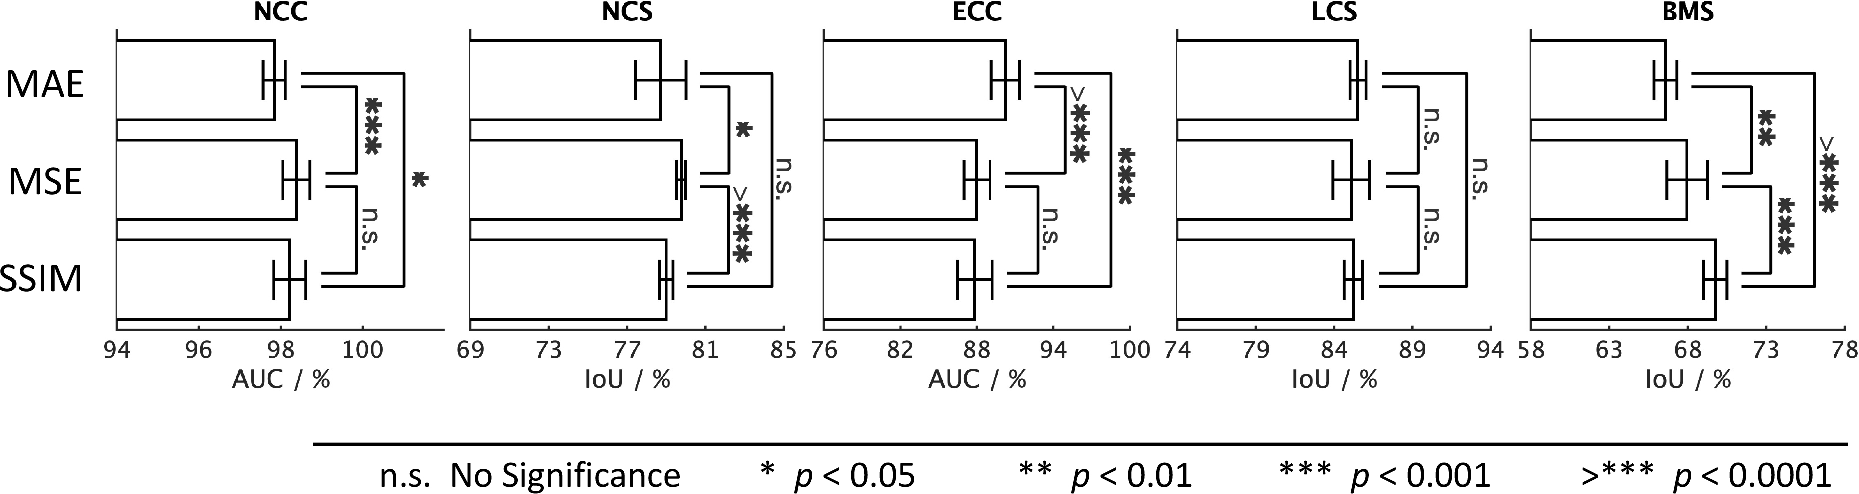
\includegraphics[width=0.9\columnwidth]{Figures/CH5/fig_losses.pdf}
\caption[Assessment the Restoration Loss and Model Transferability]{
We compare three different losses for the task of image restoration. There is no evidence that the three losses have a decisive impact on the transfer learning results of five target tasks. Note that for this ablation study, all the proxy and target tasks are implemented in PyTorch.
}
\label{ch5:fig:losses}
\end{center}
\end{sidewaysfigure}

% \fillandplacepagenumber
% \end{landscape}
%%%%%%%%%%%%%%%%%%%%%%%%%%%%%%%%%%%%%%%%%%%%

\begin{figure}[t]
\centering
\includegraphics[width=1.0\linewidth]{Figures/CH5/fig_image_restoration.pdf}
\caption[Models Genesis Can Detect Infected Regions from Images]{
Examples of image restoration using Genesis Chest CT. We pass unseen CT images (Column 1) to the pre-trained model, obtaining the restored images (Column 2). The difference between input and output has been shown in Column 3. In most of the normal cases, such as those in Rows 1---2, Genesis Chest CT can perform a fairly reasonable identical-mapping. Meanwhile, for some cases that contain opacity in the lung, as illustrated in Row 3, Genesis Chest CT tends to restore a clearer lung. As a result, the diffuse region is revealed in the difference map automatically. We have zoomed in the region for a better visualization and comparison.
}
\label{ch5:fig:image_restoration}
\end{figure}
    
    
\subsection{Does Better Restoration Transfer Better?}
\label{ch5:restoration_loss}

Our transfer learning results in Sec.~\ref{ch5:experiments} suggest that image restoration is a promising task to learn generic 3D image representation. This also means that image restoration quality has an implicit correlation with model transferability to some extent. To assess restoration quality, we compare the Mean Square Error (MSE) loss with other commonly used loss functions for image restoration\footnote{I acknowledge Jiaxuan Pang, with whom I co-authored~\citet{zhou2019models,zhou2021models}, for implementing Models Genesis in PyTorch version with Vatsal Sodha; Shivam Bajpai and Jiaxuan Pang for comparing three loss functions of the proxy task.}, such as Mean Absolute Error (MAE) and Structural Similarity Index (SSIM)~\citep{wang2004image}. All of them compute the distance between input and output images, while SSIM concentrates more on the restoration quality in terms of structural similarity than MSE and MAE. Since the publicly available 3D SSIM loss was implemented in PyTorch\footnote{\label{foot:ssim}SSIM loss in 3D: \href{https://github.com/jinh0park/pytorch-ssim-3D}{https://github.com/jinh0park/pytorch-ssim-3D}}, to make the comparisons fair, we have adapted our five target tasks into PyTorch as well. 
\figurename~\ref{ch5:fig:losses} shows mixed performances of the five target tasks among the three alternative loss functions. As discussed in Sec.~\ref{ch5:transformation_augmentation}, the ideal loss function for representation learning is one that can explicitly determine the power of image representation. However, the three losses explored in this section are implicit, based on the premise that the image restoration quality can indicate a good representation. 
Further studies with restoration quality assessment and its relationship to model transferability are therefore suggested.



\subsection{Can Models Genesis Detect Infected Regions from Images?}
\label{ch5:disease_detection}

Genesis Chest CT has been pre-trained using 623 CT images in the LUNA~2016 dataset. To assess the image restoration quality, we utilize the rest of the 265 CT images from the dataset and present examples in \figurename~\ref{ch5:fig:image_restoration}. Specifically, we pass the original CT images to the pre-trained Genesis Chest CT. To visualize the modifications, we have further plotted the difference maps by subtracting the input and output. Since the input images involve no image transformation, most of the restored CT scans (see Rows~1---2) can preserve the texture and structures of the input images, only encountering few changes thanks to the identical-mapping training scheme and the skip connections between encoder and decoder. Nonetheless, we observe some failed cases (see Row~3), especially when the input CT image contains diffuse disease, which appears as an opacity in the lung.
Genesis Chest CT happens to ``remove'' those opaque regions and restore a much clearer lung. This may be due to the fact that the majority of cropped sub-volumes are normal and are being used as ground truth, which empowers the pre-trained model with capabilities of detecting and restoring ``novelties'' in the CT scans. More specifically, in our work, these novelties include abnormal intensity distribution injected by non-linear transformation, atypical texture and boundary injected by local-shuffling, and discontinuity injected by both inner and outer cutout. Based on the surrounding anatomical structure, the model predicts the opaque area to be air, therefore restoring darker intensity values. This behavior is certainly a ``mistake'' in terms of image restoration, but it can also be thought of as an attempt to detect diffuse diseases in the lung, which is challenging to annotate due to their unclear boundary. By training an image restoration task, the diseased area will be revealed by simple \textit{subtraction} of the input and output. More importantly, this suggested detection approach requires zero human annotation, neither image-level label nor pixel-level contour, contrasting from the existing weakly supervised disease detection approaches~\citep{zhou2016learning,baumgartner2018visual,cai2018iterative,siddiquee2019learning}.


\subsection{Conclusion and Broader Impacts}
\label{ch5:discussion_conclusion:conclusion_broader_impacts}

A key contribution of ours is a collection of \textit{generic source} models, nicknamed Models Genesis, built directly from {\em unlabeled} 3D imaging data with our novel unified self-supervised method, for generating powerful application-specific \textit{target} models through transfer learning. While the empirical results are strong, surpassing state-of-the-art performances in most of the applications, our goal is to extend our Models Genesis to modality-oriented models, such as Genesis MRI and Genesis Ultrasound, as well as organ-oriented models, such as Genesis Brain and Genesis Heart. We envision that Models Genesis may serve as a primary source of transfer learning for 3D medical imaging applications, in particular, with limited annotated data. 
To benefit the research community, we make the development of Models Genesis open science, releasing our codes and models to the public. 
Creating all Models Genesis, an ambitious undertaking, takes a village; therefore, we would like to invite researchers around the world to contribute to this effort, and hope that our collective efforts will lead to the holy grail of Models Genesis, all powerful across diseases, organs, datasets, specialties, and modalities.

We first presented Models Genesis in our MICCAI 2019 paper~\citep{zhou2019models}. This paper received the MICCAI Young Scientist Award and was the Finalist for the Best Presentation Award. Models Genesis have also been chosen as one of the select contributions and received the MedIA Best Paper Award in Medical Image Analysis. This technique has been adopted for various medical imaging applications, such as lymph node classification in histopathology images~\citep{xu2020data}, COVID-19 classification in CT images~\citep{sun2020context}, brain hemorrhage classification in CT images~\citep{zhu2020aggregative}, Alzheimer's disease classification in MR images~\citep{zhang2020universal}, blood cavity segmentation in MR images~\citep{zhang2020universal}, and so on. In addition, we believe that Models Genesis would be of potential for remote sensing, given the capability of our self-supervised method learning recurrent anatomical patterns and the availability of wealthy geographical information naturally associated with satellite images.



% \section*{Acknowledgements}

% I thank Zuwei Guo for implementing Rubik's Cube~\citep{zhuang2019self} and the 3D version of Jigsaw~\citep{noroozi2016unsupervised} and DeepCluster~\citep{caron2018deep}; Fatemeh Haghighi and Mohammad Reza Hosseinzadeh Taher for implementing the 3D version of in-painting~\citep{pathak2016context}, patch-shuffling~\citep{chen2019self}, and working with Zuwei Guo in evaluating the performance of MedicalNet~\citep{chen2019med3d}; Md Mahfuzur Rahman Siddiquee for examining NiftyNet~\citep{gibson2018niftynet} with our Models Genesis; Pengfei Zhang for comparing two additional random initialization methods with our Models Genesis; Shivam Bajpai for comparing three loss functions of the proxy task; Nima Tajbakhsh for revising our conference paper; Jae Y. Shin for organizing and pre-processing the PE dataset; Ruibin Feng for valuable discussions; and Keerthi Shrikar Tatapudi for helping improve the writing of this paper.